\section*{Appendix}


\if 0
\subsection*{A1:  Display Power of Same UI Varies with the Phones}

\begin{figure}[]
	\begin{tabular}[]{ l r }
 	\begin{subfigure}[]{0.35\columnwidth}
 		\frame{\includegraphics[width=\textwidth]{./figure/900_BASE_Model_Comparision.png}}
 		\caption{Original}
 	\end{subfigure}
 	\begin{subfigure}[]{0.35\columnwidth}
 		\frame{\includegraphics[width=\textwidth]{./figure/901_N6_Model_Comparision.png}}
 		\caption{Nexus 6}
 	\end{subfigure}
	&
	\multirow{2}{*}{
 	\begin{subfigure}[]{0.15\columnwidth}
 		\includegraphics[width=\textwidth]{./figure/904_Current_Model_Comparision.png}
 		\caption{Current\\(in mA)}
 	\end{subfigure}} \\
 	\begin{subfigure}[]{0.35\columnwidth}
 		\frame{\includegraphics[width=\textwidth]{./figure/903_P2_Model_Comparision.png}}
 		\caption{Pixel 2}
 	\end{subfigure}
 	\begin{subfigure}[]{0.35\columnwidth}
 		\frame{\includegraphics[width=\textwidth]{./figure/902_Z3_Model_Comparision.png}}
 		\caption{Moto Z3}
 	\end{subfigure}	
	& \\
	\end{tabular}
        \vspace{-0.1in}
	\caption{Pixel power draw distribution for the same Message App
          screen shot on the three phones. The estimated total
          display power are 294 mA for Nexus 6, 232 mA for Pixel 2,
          and 309 mA for Moto Z3.}
        \vspace{-0.1in}
	\label{fig:oled_model_comparison}
\end{figure}

We first show that it is easy to measure and show that the OLED
display power for different phones can differ while displaying the base
colors (red/green/blue), \eg using a powermeter or in-built power
sensor.
Our accurate OLED display power estimation allows the developer to see how the
OLED power differ for any complex frame or image for different phones.

As an illustrstion, we captured a screen shot in playing the Google
Message App (Figure~\ref{fig:oled_model_comparison}(a)). This screen
has both dark and bright regions. We next applied our PWLM power
models for the 3 phones to estimate the power consumed by every
pixel in the captured screen shot. In fact, we built a program that
superimposes the resulting pixel power distribution as a heat map of the
original image.  Figures~\ref{fig:oled_model_comparison}(b)-(d) shows
the output of the program for the 3 phones.  We easily see from the heap map that for
the top white portion of the screen for Moto Z3's OLED display consumes
the most power, followed by Nexus 6 and Pixel 2.

The difference in OLED power draw by the 3 phones can be
attributed to the different OLED technologies (see
Table~\ref{tab:phones}) and possibly different
OLED circuitry. The variation in power draw also motivates the need to
derive OLED display power for every handset.
\fi

\if 0
Active Matrix Organic Light Emitting Diodes or AMOLED display
technology consists of an array of closely integrated OLED to create
the content on our display.  Plastic-OLED or P-OLED is a special kind
of AMOLED which has lower power consumption in comparision to earlier
used AMOLED.

To show the difference between OLED and P-OLED current consumptions we 
generated a heat map. The Figure\ref{fig:oled_model_comparison} shows
the heat map for Nexus 6 (in (b)),PIXEL2 (on (d)) and the original image (on (a)).

The screens of Nexus 6 and PIXEL2 while displaying brighter colors
(i.e. towards red) represents higher OLED current consumption and while
displying cooler colors (i.e. towards blue) represents lower OLED current
consumption. We can clearly observe from the figure that PIXEL2 OLED
display consumes much less current compared to current consumed by
Nexus 6 display. Further we estimated that while Nexus 6 average
cureent consumption is  about 352mA , the averages current consumption
of PIXEL2 is less i.e about 283mA.

From this we can conclude that future trend in OLED technology is
likely to further decrease screen power consumption.


\fi

\subsection*{A1: Power Saving of App Activities for the Remaining Apps}

We discuss how dark mode helps to save OLED power for major activities 
in Google Calculator, Google Calender, Google Phone, Google Maps, and YouTube below.

\begin{figure}[h]
	\begin{subfigure}[]{\columnwidth}
		\centering
		% 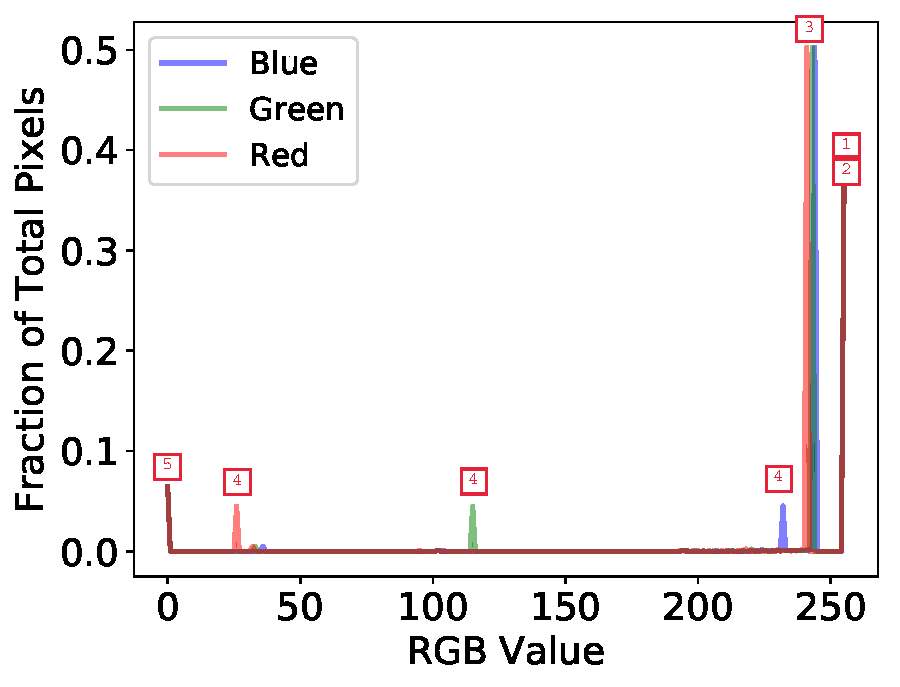
\includegraphics[width=0.58\columnwidth]{./figure/601a_calculator_light.pdf}\quad
		% \frame{\includegraphics[width=0.27\columnwidth]{./figure/651_calculator_light.png}}
		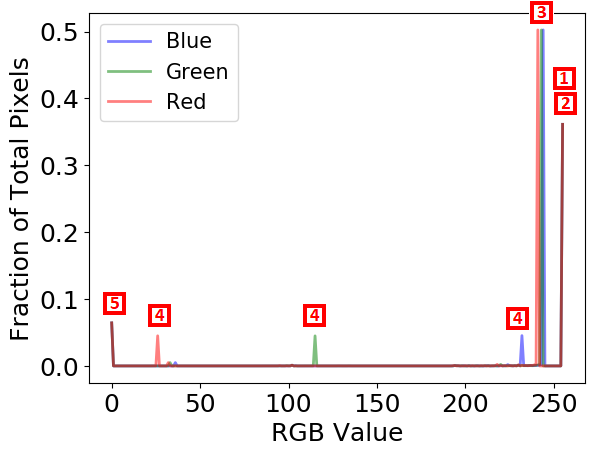
\includegraphics[width=0.58\columnwidth]{./figure/601a_calculator_light.png}\quad
		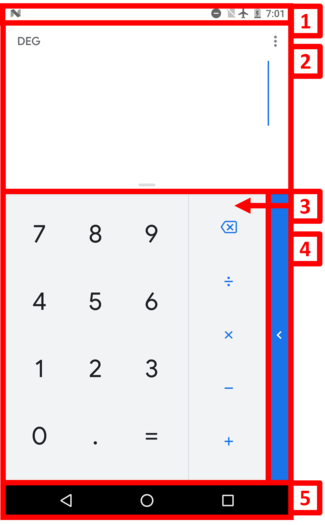
\includegraphics[width=0.27\columnwidth]{./figure/651a_calculator_light.png}
		\caption{Light mode}
	\end{subfigure}
	\begin{subfigure}[]{\columnwidth}
		\centering
		% \includegraphics[width=0.58\columnwidth]{./figure/600a_calculator_dark.pdf}\quad
		% \frame{\includegraphics[width=0.27\columnwidth]{./figure/650_calculator_dark.png}}
		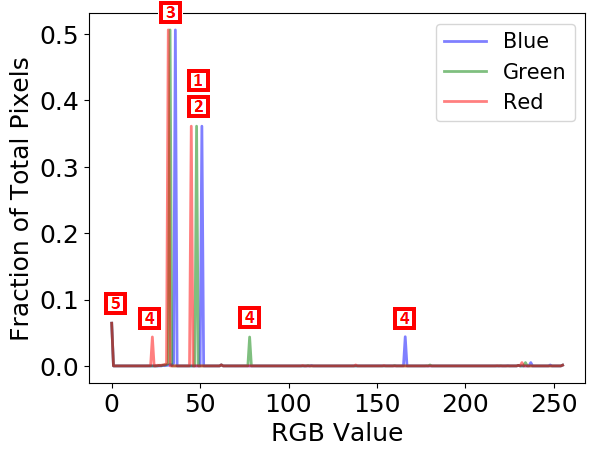
\includegraphics[width=0.58\columnwidth]{./figure/600a_calculator_dark.png}\quad
		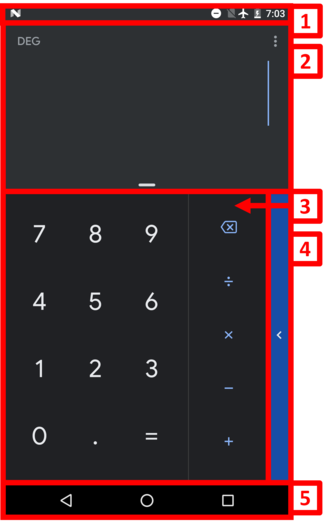
\includegraphics[width=0.27\columnwidth]{./figure/650a_calculator_dark.png}
		\caption{Dark mode}
	\end{subfigure}
	\\
	\begin{subfigure}[]{\columnwidth}
	\centering
	{ \small
	\begin{tabular}{ | l | r | r | r |}
		\hline
		     & \multicolumn{3}{|c|}{Power Reduction (mA)}\\
		\cline{2-4}
                Part   & Nexus 6 & Pixel 2 & Moto Z3 \\
		\hline
		1 &   8 &   10 &   13  \\
		2 &  73 &   92 &  122  \\
		3 & 111 &  133 &  178  \\
		4 &   4 &    3 &    4  \\
		5 &   0 &    0 &    0  \\
		\hline
		Total   & 196 & 238 & 317  \\
		\hline
	\end{tabular}
	}
	\caption{OLED power saving}
        \vspace{-0.1in}
	\end{subfigure}
	\caption{Google Calculator: Home activity}
	\label{fig:case_study_calculator}
\end{figure}

{\bf Google Calculator.}
% This is like many other apps which has only text in it like
% Contacts and does not contain Messages (with images) and other contents.
Figure~\ref{fig:case_study_calculator} shows the screenshots of the home
activity of Caculator (right) and the histogram of the RGB values of
all its pixels (left) under light and dark modes.  We see that the
activity screen can be divided into 5 parts. The Status bar (part 1)
and upper part of the screen (part 2) have identical white color 
(corresponding to the peaks with RGB values of 256 in the histogram).
In dark mode, both peaks move to the dark side (with identical RGB values of 50),
which results in 8mA/10mA/13mA (on 3 phones) power saving for the Status Bar and
73mA/92mA/122mA saving for part 2.
% We observed this trend in many
% apps where status bar takes the identical color of app's upper part.
Part 3 is the second major chunk of the screen which corresponds to the
keyboard.  In changing from the light to dark mode, its
corresponding peak in the histogram moves from RGB value 241-246  to 31-37,
saving 111mA/133mA/178mA.
%
Finally, the Navigation bar (part 5) is black in both modes
and does not save power in dark mode,
and side bar (part 4) stays in close-to-dark
color in both modes, saving about 4mA/3mA/4mA.
Summing up the power savings from all 5 parts 
gives a total power saving of 196mA/238mA/317mA
on the three phones, respectively (Figure~\ref{fig:case_study_calculator}(c)).

\begin{figure}[h]
	\begin{subfigure}[]{\columnwidth}
		\centering
		% \includegraphics[width=0.58\columnwidth]{./figure/611_phone_light.pdf}\quad
		% \frame{\includegraphics[width=0.27\columnwidth]{./figure/661_phone_light.png}}
		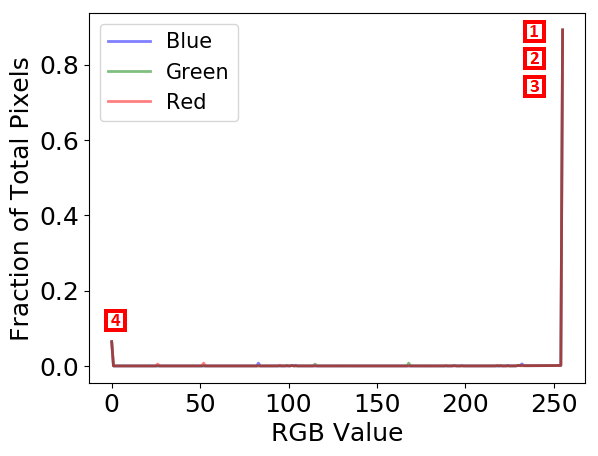
\includegraphics[width=0.58\columnwidth]{./figure/611a_phone_light.png}\quad
		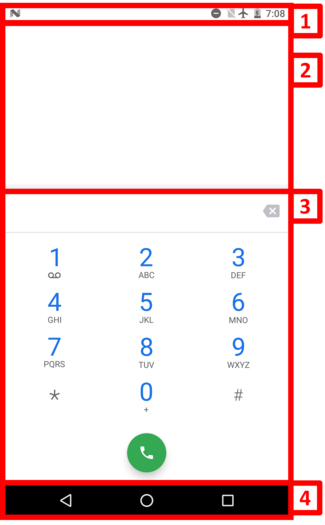
\includegraphics[width=0.27\columnwidth]{./figure/661a_phone_light.png}
		\caption{Light mode}
	\end{subfigure}
	\begin{subfigure}[]{\columnwidth}
		\centering
		% \includegraphics[width=0.58\columnwidth]{./figure/610_phone_dark.pdf}\quad
		% \frame{\includegraphics[width=0.27\columnwidth]{./figure/660_phone_dark.png}}
		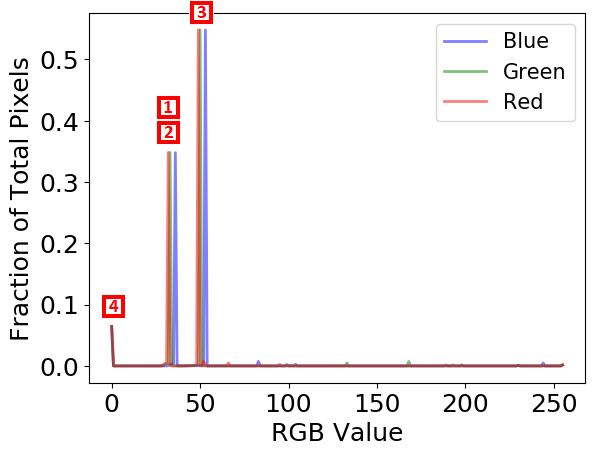
\includegraphics[width=0.58\columnwidth]{./figure/610a_phone_dark.png}\quad
		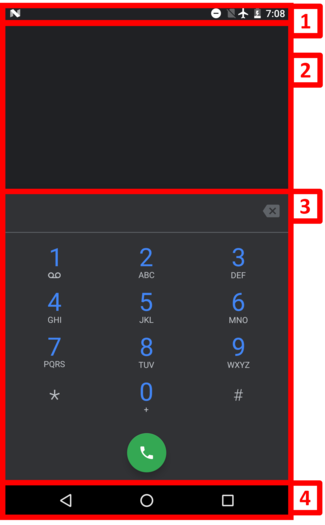
\includegraphics[width=0.27\columnwidth]{./figure/660a_phone_dark.png}
		\caption{Dark mode}
	\end{subfigure}
	\\
	\begin{subfigure}[]{\columnwidth}
	\centering
	{ \small
	\begin{tabular}{ | l | r | r | r | }
		\hline
		     & \multicolumn{3}{|c|}{Power Reduction (mA)}\\
		\cline{2-4}
                Part & Nexus 6 & Pixel 2 & Moto Z3 \\
		\hline
		1 &   8  &  10 &   13  \\
		2 &  78  &  97 &  129  \\
		3 & 126  & 161 &  212  \\
		4 &   0  &   0 &    0  \\
		\hline
		Total   & 212 & 268 & 354  \\
		\hline
	\end{tabular}
	}
	\caption{OLED power saving}
        \vspace{-0.1in}
	\end{subfigure}
	\caption{Phone: Main activity.}
	\label{fig:case_study_phone}
\end{figure}

{\bf Google Phone.} Figure~\ref{fig:case_study_phone} shows that the
main activity screen of this app is very similar to that of Calculator,
and consist of 4 parts: Status Bar (part 1), upper part (part 2), Dial
number part (part 3), and Navigation bar (part 4).  The first 3 parts
switch from white color in the light mode to near-dark colors (with
RGB values around 50) in the dark mode, which result in significant
OLED power saving (Figure~\ref{fig:case_study_phone}(c)).

\begin{figure}[h]
	\begin{subfigure}[]{\columnwidth}
		\centering
		% \includegraphics[width=0.58\columnwidth]{./figure/603_calender_light.pdf}\quad
		% \frame{\includegraphics[width=0.27\columnwidth]{./figure/653_calender_light.png}}
		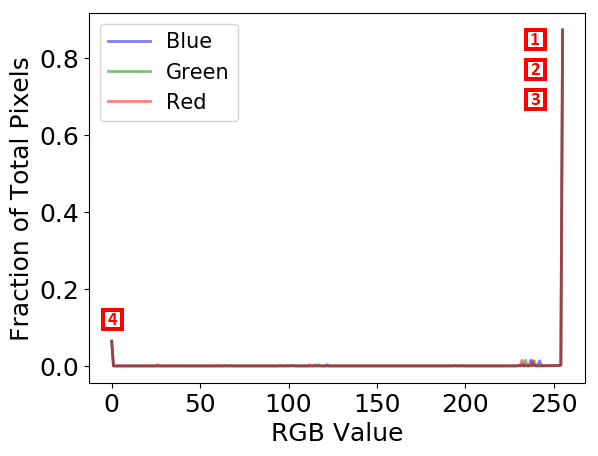
\includegraphics[width=0.58\columnwidth]{./figure/603a_calender_light.png}\quad
		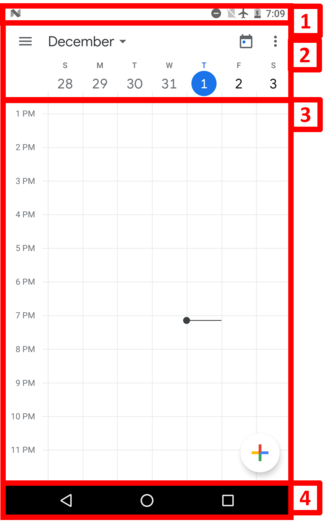
\includegraphics[width=0.27\columnwidth]{./figure/653a_calender_light.png}
		\caption{Light mode}
	\end{subfigure}
	\begin{subfigure}[]{\columnwidth}
		\centering
		% \includegraphics[width=0.58\columnwidth]{./figure/602_calender_dark.pdf}\quad
		% \frame{\includegraphics[width=0.27\columnwidth]{./figure/652_calender_dark.png}}
		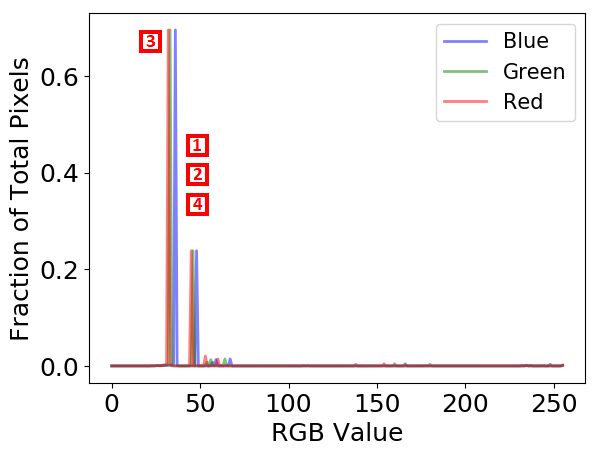
\includegraphics[width=0.58\columnwidth]{./figure/602a_calender_dark.png}\quad
		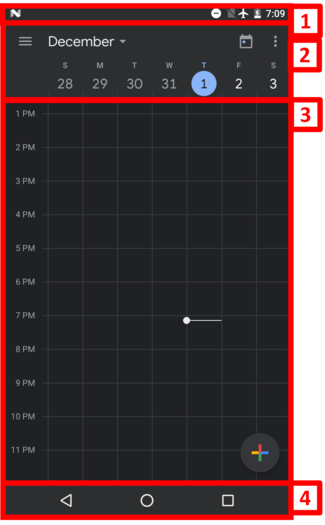
\includegraphics[width=0.27\columnwidth]{./figure/652a_calender_dark.png}
		\caption{Dark mode}
	\end{subfigure}
	\\
	\begin{subfigure}[]{\columnwidth}
	\centering
	{ \small
	\begin{tabular}{ | l | r | r | r | }
		\hline
		     & \multicolumn{3}{|c|}{Power Reduction (mA)}\\
		\cline{2-4}
                Part & Nexus 6 & Pixel 2 & Moto Z3 \\
		\hline
		1 &     9 &    11 &    14  \\
		2 &    31 &    39 &    52  \\
		3 &   173 &   216 &   287  \\
		4 & -0.09 &  -0.4 &  -0.3  \\
		\hline
		Total   & 213 & 266 & 353  \\
		\hline
	\end{tabular}
	}
	\caption{OLED power saving}		
        \vspace{-0.1in}
	\end{subfigure}
	\caption{Google Calender: Main activity.}
	\label{fig:case_study_calender}
\end{figure}

{\bf Google Calender.} Figure~\ref{fig:case_study_phone} shows that the
main activity screen of this app is very similar to that of Calculator,
and consist of 4 parts: Status Bar (part 1), Weekly view (part 2), Day
view part (part 3), and Navigation bar (part 4).  The first 3 parts
switch from white color in the light mode to near-dark colors (with
RGB values around 50) in the dark mode, which result in significant
OLED power saving (Figure~\ref{fig:case_study_calender}(c)).
Interestingly, part 4 switched from dark color in the light mode
to near-dark color (RGB value of (44,44,44)) in the dark mode which increases
its power draw slightly.


\begin{figure}[tp]
	\begin{subfigure}[]{\columnwidth}
		\centering
		% \includegraphics[width=0.58\columnwidth]{./figure/607_maps_light.pdf}\quad
		% \frame{\includegraphics[width=0.27\columnwidth]{./figure/657_maps_light.png}}
		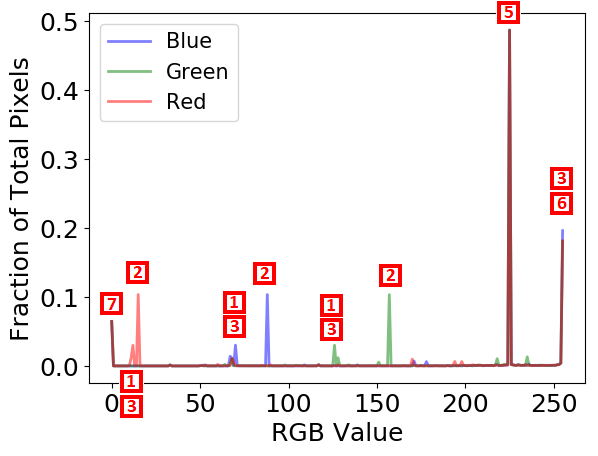
\includegraphics[width=0.58\columnwidth]{./figure/607a_maps_light.png}\quad
		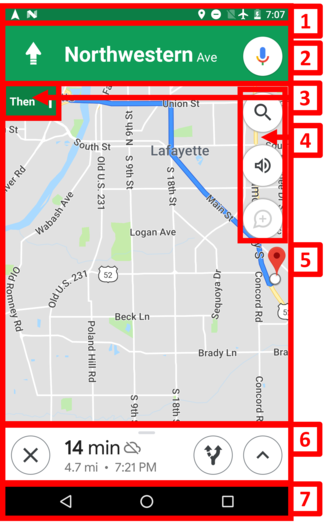
\includegraphics[width=0.27\columnwidth]{./figure/657a_maps_light.png}
		\caption{Light mode}
	\end{subfigure}
	\begin{subfigure}[]{\columnwidth}
		\centering
		% \includegraphics[width=0.58\columnwidth]{./figure/606_maps_dark.pdf}\quad
		% \frame{\includegraphics[width=0.27\columnwidth]{./figure/656_maps_dark.png}}
		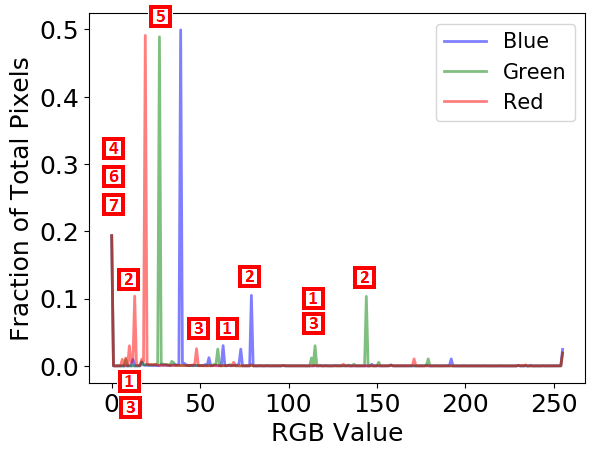
\includegraphics[width=0.58\columnwidth]{./figure/606a_maps_dark.png}\quad
		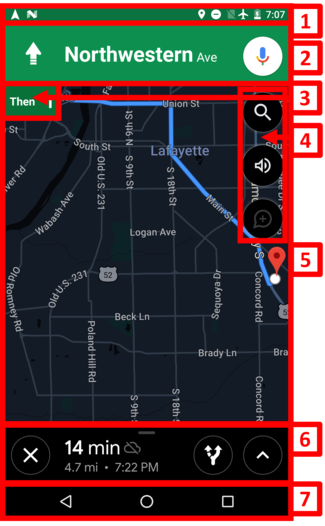
\includegraphics[width=0.27\columnwidth]{./figure/656a_maps_dark.png}
		\caption{Dark mode}
	\end{subfigure}
	\\
	\begin{subfigure}[]{\columnwidth}
	\centering
	{ \small
	\begin{tabular}{ | l | r | r | r | }
		\hline
		     & \multicolumn{3}{|c|}{Power Reduction (mA)}\\
		\cline{2-4}
                Part & Nexus 6 & Pixel 2 & Moto Z3 \\
		\hline
		1 & 0.2  & 0.2  & 0.2  \\
		2 & 0.8  & 0.8  &   1  \\
		3 & 0.2  & 0.2  & 0.3  \\
		4 &  10  &  12  &  16  \\
		5 & 113  & 132  & 175  \\
		6 &  24  &  31  &  41  \\
		7 &   0  &   0  &   0  \\
		\hline
		Total   & 148 &  176 &  234  \\
		\hline
	\end{tabular}
	}
	\caption{OLED power saving}		
        \vspace{-0.1in}
	\end{subfigure}
	\caption{Google Maps: Navigation activity.}
	\label{fig:case_study_maps}
\end{figure}

Figure~\ref{fig:case_study_maps} shows
that Google Map main activity is dominated
by the dynamically changing map (part 5),
consisting of roads and blocks which
change from white to dark grey in switching from the light to dark mode,
and shift the peak from around 255 to 21 - 39 in the histograms.
%  These represent two distinctive peaks. 
%  The total display power saving by dark mode of Google Map app is 139mA/164mA/217mA.
The activity screen is rich in UI design and consists 6 other parts:
Status Bar (1),
street name (2),
navigation sign (3),
utility icons (4),
driving stats (6),
and Navigation Bar (7).
The major power saving (Figure~\ref{fig:case_study_maps}(c))
comes from parts 4, 5, 6, which switch from
white or near-white color to dark (parts 4 and 6) and near-dark color (part 5).
The remaining 4 parts, in particular, the street name display (part 2), do not
change color and save close-to-zero power.

\begin{figure}[h]
	\begin{subfigure}[]{\columnwidth}
		\centering
		% \includegraphics[width=0.58\columnwidth]{./figure/613_youtube_light.pdf}\quad
		% \frame{\includegraphics[width=0.27\columnwidth]{./figure/663_youtube_light.png}}
		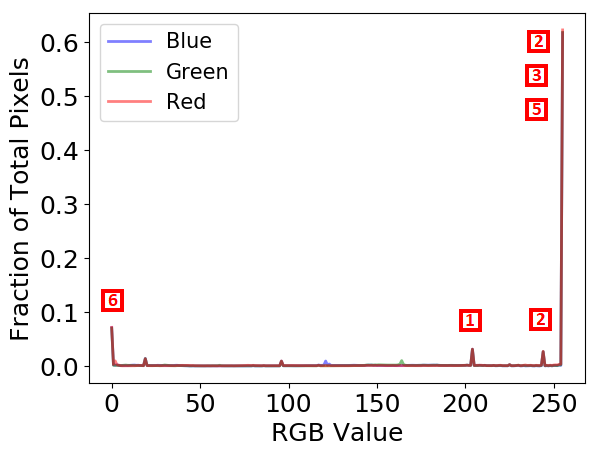
\includegraphics[width=0.58\columnwidth]{./figure/613a_youtube_light.png}\quad
		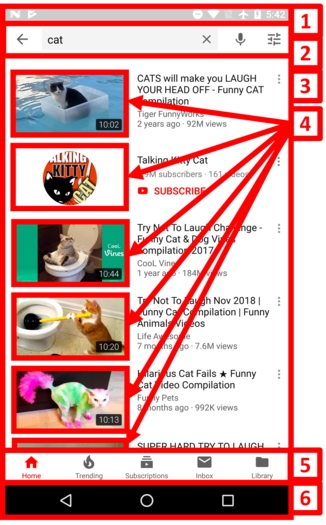
\includegraphics[width=0.27\columnwidth]{./figure/663a_youtube_light.png}
		\caption{Light mode}
	\end{subfigure}
	\begin{subfigure}[]{\columnwidth}
		\centering
		% \includegraphics[width=0.58\columnwidth]{./figure/612_youtube_dark.pdf}\quad
		% \frame{\includegraphics[width=0.27\columnwidth]{./figure/662_youtube_dark.png}}
		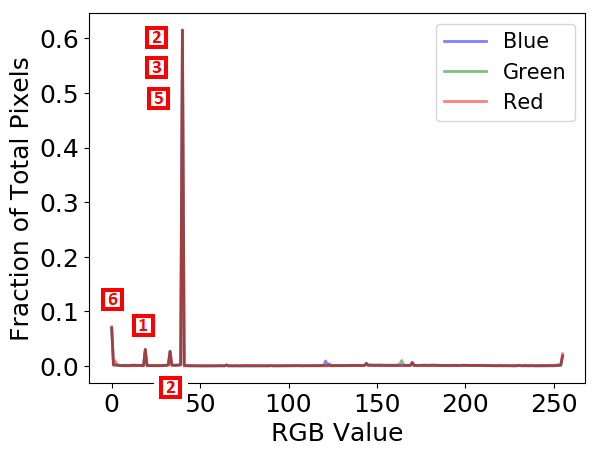
\includegraphics[width=0.58\columnwidth]{./figure/612a_youtube_dark.png}\quad
		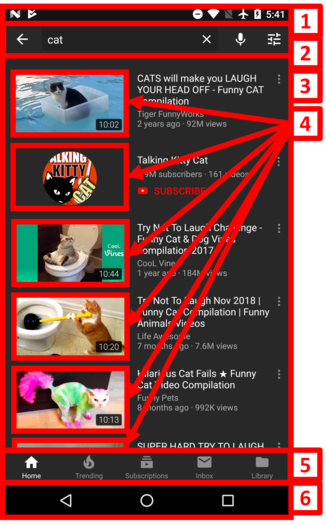
\includegraphics[width=0.27\columnwidth]{./figure/662a_youtube_dark.png}
		\caption{Dark mode}
	\end{subfigure}
	\\
	\begin{subfigure}[]{\columnwidth}
	\centering
	{ \small
	\begin{tabular}{ | l | r | r | r | }
		\hline
		     & \multicolumn{3}{|c|}{Power Reduction (mA)}\\
		\cline{2-4}
                Part & Nexus 6 & Pixel 2 & Moto Z3 \\
		\hline
		1 &   6 &     6 &    8  \\
		2 &  15 &    18 &   24  \\
		3 & 120 &   151 &  200  \\
		4 &   0 &     0 &    0  \\
		5 &  13 &    17 &   22  \\
		6 &   0 &     0 &    0  \\
		\hline
		Total   & 154 & 192 & 254  \\
		\hline
	\end{tabular}
	}
	\caption{OLED power saving}		
        \vspace{-0.1in}
	\end{subfigure}
	\caption{YouTube: Home activity.}
	\label{fig:case_study_youtube}
\end{figure}

{\bf YouTube.}  Figure~\ref{fig:case_study_youtube}(a) shows tha the
browsing activity of YouTube is similar to that of Google News -- the
majority of the screen is occupied with the search results (part 3)
along with video clip images (part 4).  Consequently, the search
result section contributes to most of the OLED power saving in
switching from white color in the light mode to near-dark color (RGB
value of 40) in dark mode
(Figure~\ref{fig:case_study_youtube}(c)).  As with other
apps, the Seacrch bar (part 2), status bar (part 1), and
YouTube menu (part 5) also contribute to the OLED power saving from
switching to near-dark color. The list of images, whose pixels are
spread over the whole color space and hence not visible as any peaks in
the histogram, do not contribute to any OLED power reduction.


\subsection*{A2: Color Modes and the linear property}

Figure\ref{fig:initial_evaluation_color_mode}
shows the OLED power draw in displaying monochromatic images on
for non-default color modes on Pixel 2 and Moto Z3.
We see that the power draw for the same linear RGB value differs from
those for the default mode in Figure~\ref{fig:initial_evaluation_2}
due to color transformation in HardwareComposer.
Hence, a new OLED power model needs to be generated for each color mode.

%  also shows that the code mode does differ from each other vastly
%  like PIXEL 2 natural and saturated as seen in Figure\ref{fig:initial_evaluation_color_mode}(a)(b).

\begin{figure*}[tp]
	\begin{subfigure}[]{0.31\textwidth}
		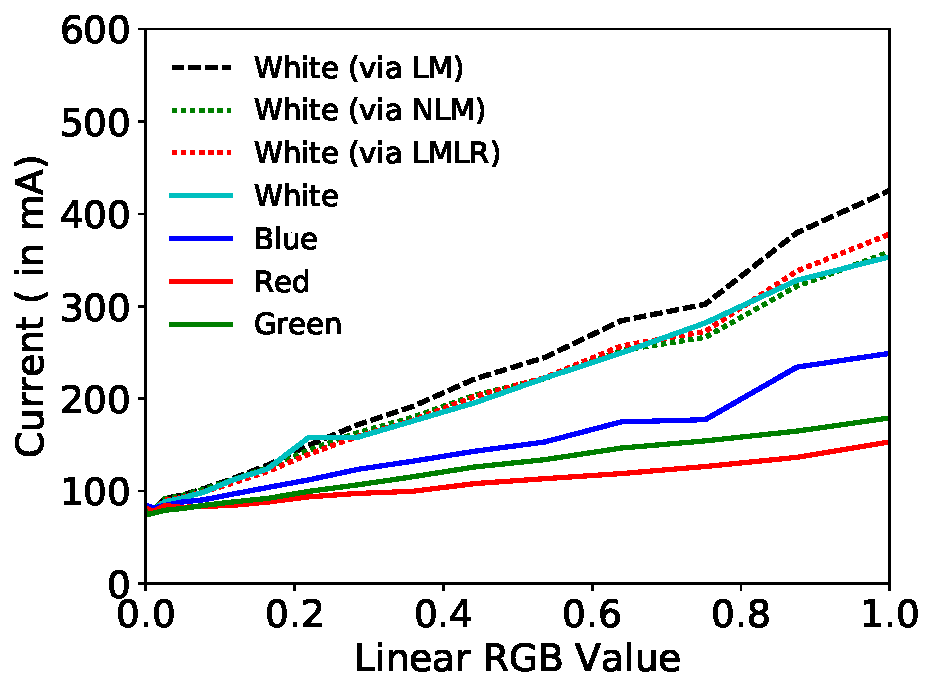
\includegraphics[width=\textwidth]{./figure/1602_P2_Natural_White.pdf}
		\caption{Pixel 2: Natural Color Mode for white}
		\label{fig:initial_evaluation_2_n6_w_c}
	\end{subfigure}
	\hfill
	\begin{subfigure}[]{0.31\textwidth}
		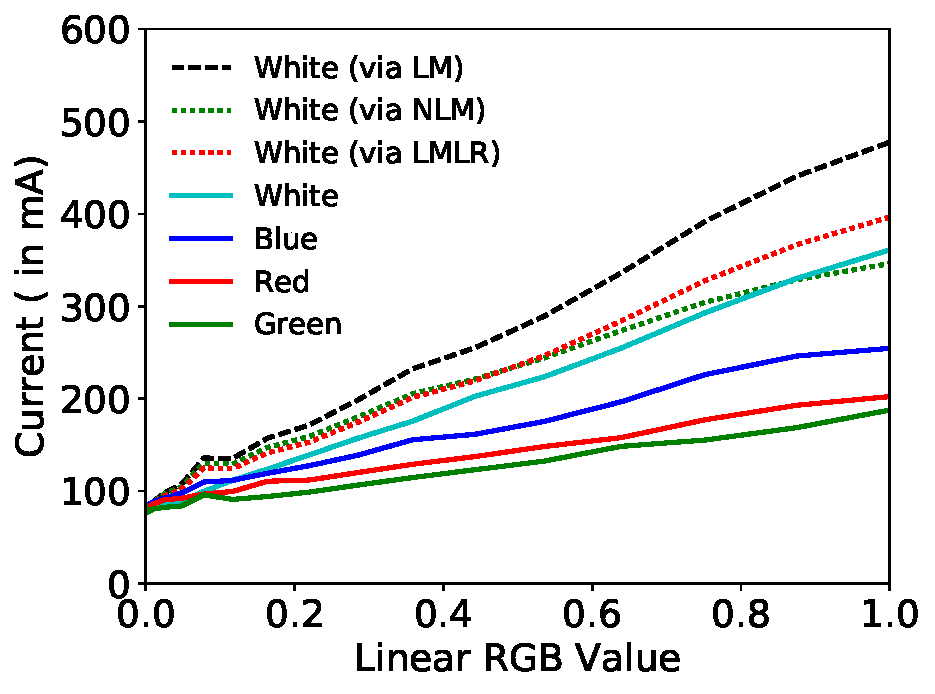
\includegraphics[width=\textwidth]{./figure/1600_P2_Saturated_White.pdf}
		\caption{Pixel 2: Saturated Color mode for white}
		\label{fig:initial_evaluation_2_p2_w_c}
	\end{subfigure}
	\hfill
	\begin{subfigure}[]{0.31\textwidth}
		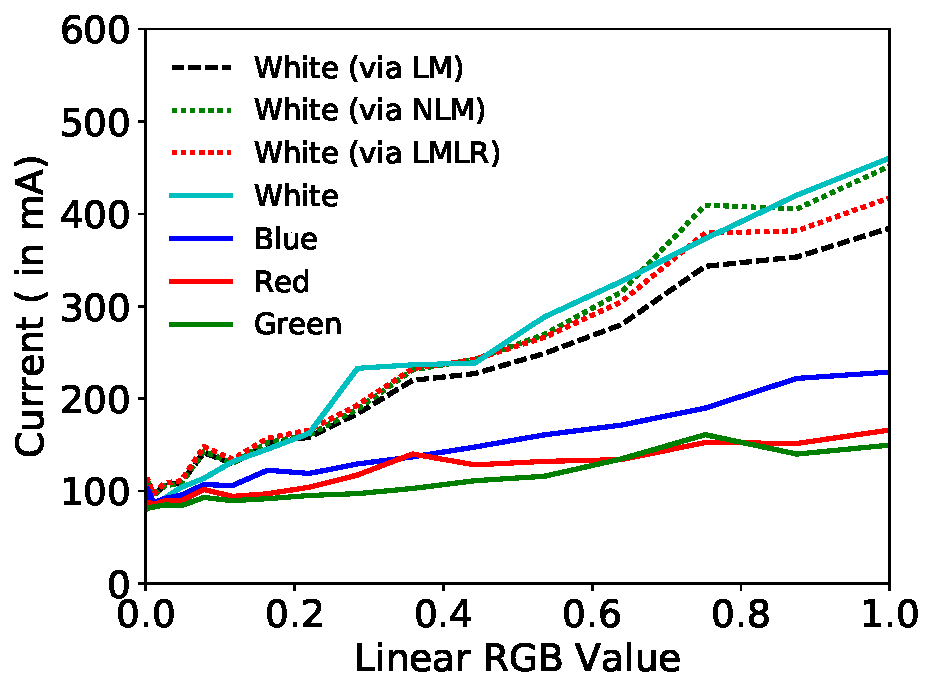
\includegraphics[width=\textwidth]{./figure/1603_Z3_Standard_White.pdf}
		\caption{Moto Z3: Standard Color Mode for white}
		\label{fig:initial_evaluation_2_z3_w_c}
	\end{subfigure}
\\
	\begin{subfigure}[]{0.31\textwidth}
		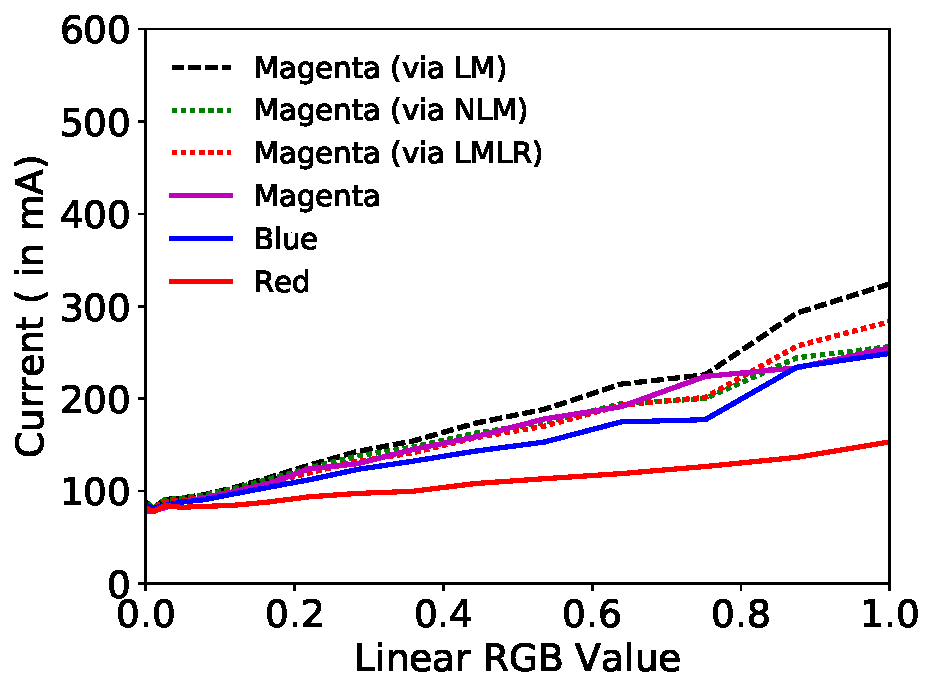
\includegraphics[width=\textwidth]{./figure/1632_P2_Natural_Magenta.pdf}
		\caption{Pixel 2: Natural Color Mode}
		\label{fig:initial_evaluation_2_n6_m_c for magenta}
	\end{subfigure}
        \hfill
	\begin{subfigure}[]{0.31\textwidth}
		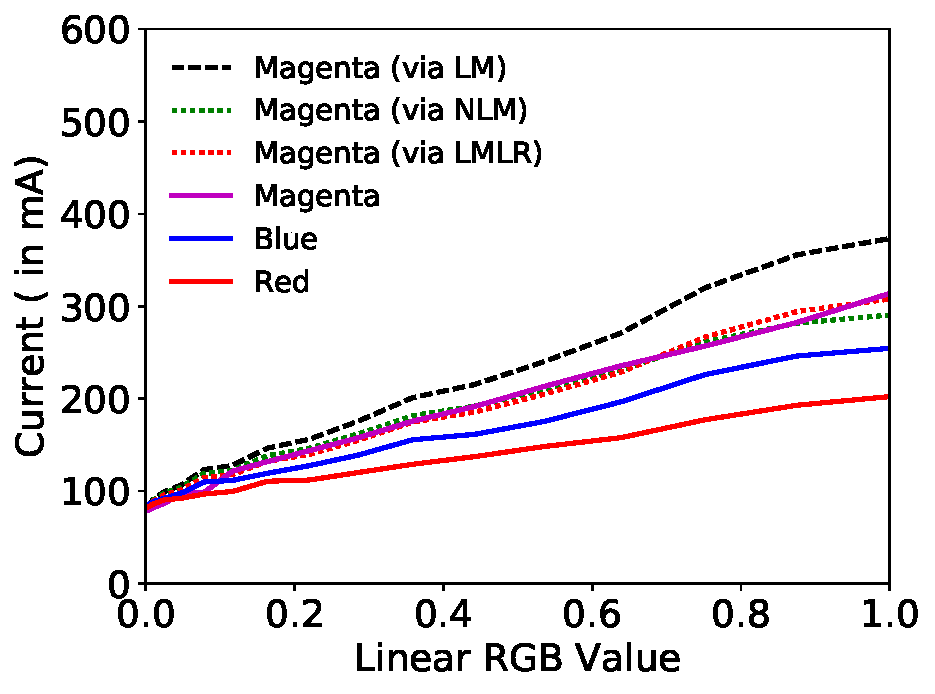
\includegraphics[width=\textwidth]{./figure/1631_P2_Saturated_Magenta.pdf}
		\caption{Pixel 2: Saturated Color mode for magenta}
		\label{fig:initial_evaluation_2_p2_m_c}
	\end{subfigure}
        \hfill
	\begin{subfigure}[]{0.31\textwidth}
		\includegraphics[width=\textwidth]{./figure/1633_Z3_Standard_Magenta.pdf}
		\caption{Moto Z3: Standard Color Mode for magenta}
		\label{fig:initial_evaluation_2_z3_m_c}
	\end{subfigure}
        \vspace{-0.1in}
	\caption{OLED display power in displaying one-color images on three phones
		for non default color modes.
		(LM: linear model as in Eqn.\ref{eq:linear_equation0},
		 LMLR: linear model with linear regression, NLM: Non-Linear Model)
		}
%        \vspace{-0.1in}
        \label{fig:initial_evaluation_color_mode}
\end{figure*}

\subsection*{A3: Impact of Subgrid Size on New Model Accuracy}

Figures~\ref{fig:100_images_expriment2}(a)-(c) show the CDF of
prediction error of P-LMLR and P-NLM models across the 100 images
under subgrid sizes 16 and 32, on the three phones, respectively.
We see that the prediction errors are very similar on the 3 phones.

\begin{figure*}[tp]
	\begin{subfigure}[]{0.29\textwidth}
		\includegraphics[width=\textwidth]{./figure/1000_N6_100_image_error_cdf.pdf}
        \vspace{-0.1in}
		\caption{Nexus 6}
	\end{subfigure}
	\begin{subfigure}[]{0.29\textwidth}
		\includegraphics[width=\textwidth]{./figure/1002_P2_100_image_error_cdf.pdf}
        \vspace{-0.1in}
		\caption{Pixel 2}
	\end{subfigure}
	\begin{subfigure}[]{0.29\textwidth}
		\includegraphics[width=\textwidth]{./figure/1001_Z3_100_image_error_cdf.pdf}
        \vspace{-0.1in}
		\caption{Moto Z3}
	\end{subfigure}
        \vspace{-0.1in}
	\caption{Impact of subgrid size on the prediction accuracy of P-LMLR and P-NLM models
          for the 100 images.}
	\label{fig:100_images_expriment2}
\end{figure*}

